\documentclass{article}

\usepackage{noweb}
\noweboptions{smallcode,longchunks}
\usepackage[a4paper,margin=1in]{geometry}
\usepackage{colortbl}
\usepackage[colorlinks=true]{hyperref}
\usepackage{tikz}

\newcommand{\hi}[1]{\noindent {\bf #1}}     % Define a handy paragraph opener

\def\nwendcode{\endtrivlist \endgroup}      % Remove noweb page break penalty
\let\nwdocspar=\par

\title{Jargo Distance Utilities\footnote{
  \url{https://github.com/jargors/Tools}}}
\author{James J. Pan\\
  \small{\href{mailto:pan-j16@mails.tsinghua.edu.cn}{pan-j16@mails.tsinghua.edu.cn}}}

\begin{document}
\maketitle
\pagestyle{noweb}

\tableofcontents

\section{Introduction}
\label{sec:introduction}
We supply a Tools class that provides some common procedures for developing
ridesharing algorithms.  The Tools class is developed using the
Noweb\footnote{\url{https://www.cs.tufts.edu/~nr/noweb/}} literate
programming\footnote{\url{http://literateprogramming.com/}} tool.  This file
({\tt{}src/Tools.nw}) is the source for both the documentation ({\tt{}doc/Tools.tex})
and the Java code (Tools.java)\footnote{See the {\tt{}Makefile} for build
details.}.

\section{Implementation Overview}
\nwfilename{src/Tools.nw}\nwbegincode{1}\sublabel{NW3zOIuJ-2Vh5vZ-1}\nwmargintag{{\nwtagstyle{}\subpageref{NW3zOIuJ-2Vh5vZ-1}}}\moddef{Tools.java~{\nwtagstyle{}\subpageref{NW3zOIuJ-2Vh5vZ-1}}}\endmoddef\nwnotused{Tools.java}
\LA{}Tools.java preamble~{\nwtagstyle{}\subpageref{NW3zOIuJ-1ANZ96-1}}\RA{}
\LA{}\code{}Tools\edoc{} definition~{\nwtagstyle{}\subpageref{NW3zOIuJ-1xm30x-1}}\RA{}
\nwendcode{}\nwbegindocs{2}\nwdocspar

\subsection{Preamble}
The preamble declares the package and imports dependencies.
\nwenddocs{}\nwbegincode{3}\sublabel{NW3zOIuJ-1ANZ96-1}\nwmargintag{{\nwtagstyle{}\subpageref{NW3zOIuJ-1ANZ96-1}}}\moddef{Tools.java preamble~{\nwtagstyle{}\subpageref{NW3zOIuJ-1ANZ96-1}}}\endmoddef\nwused{\\{NW3zOIuJ-2Vh5vZ-1}}
package com.github.jargors;
import com.github.jargors.gtreeJNI.*;
import java.util.Map;
import java.util.HashMap;
import java.util.Arrays;
\nwendcode{}\nwbegindocs{4}\nwdocspar

\subsection{Class Definition}
\nwenddocs{}\nwbegincode{5}\sublabel{NW3zOIuJ-1xm30x-1}\nwmargintag{{\nwtagstyle{}\subpageref{NW3zOIuJ-1xm30x-1}}}\moddef{\code{}Tools\edoc{} definition~{\nwtagstyle{}\subpageref{NW3zOIuJ-1xm30x-1}}}\endmoddef\nwused{\\{NW3zOIuJ-2Vh5vZ-1}}
public class Tools \{
  \LA{}Member variables~{\nwtagstyle{}\subpageref{NW3zOIuJ-aPohW-1}}\RA{}
  \LA{}Public methods~{\nwtagstyle{}\subpageref{NW3zOIuJ-1eKCCy-1}}\RA{}
\}
\nwendcode{}\nwbegindocs{6}\nwdocspar

\subsection{Member Variables}
\nwenddocs{}\nwbegincode{7}\sublabel{NW3zOIuJ-aPohW-1}\nwmargintag{{\nwtagstyle{}\subpageref{NW3zOIuJ-aPohW-1}}}\moddef{Member variables~{\nwtagstyle{}\subpageref{NW3zOIuJ-aPohW-1}}}\endmoddef\nwused{\\{NW3zOIuJ-1xm30x-1}}
private G_Tree gtree;
private boolean flag_gtree_loaded = false;
private Map<Integer, int[]> lu_vertices = new HashMap<>();
private Map<Integer, Map<Integer, int[]>> lu_edges = new HashMap<>();
private Map<Integer, int[]> lu_users = new HashMap<>();
private final double CSHIFT = 10000000.0;
\nwindexdefn{gtree}{gtree}{NW3zOIuJ-aPohW-1}\nwindexdefn{flag{\char95}gtree{\char95}loaded}{flag:ungtree:unloaded}{NW3zOIuJ-aPohW-1}\nwindexdefn{lu{\char95}vertices}{lu:unvertices}{NW3zOIuJ-aPohW-1}\nwindexdefn{lu{\char95}edges}{lu:unedges}{NW3zOIuJ-aPohW-1}\nwindexdefn{lu{\char95}users}{lu:unusers}{NW3zOIuJ-aPohW-1}\nwindexdefn{CSHIFT}{CSHIFT}{NW3zOIuJ-aPohW-1}\eatline
\nwidentdefs{\\{{CSHIFT}{CSHIFT}}\\{{flag{\char95}gtree{\char95}loaded}{flag:ungtree:unloaded}}\\{{gtree}{gtree}}\\{{lu{\char95}edges}{lu:unedges}}\\{{lu{\char95}users}{lu:unusers}}\\{{lu{\char95}vertices}{lu:unvertices}}}\nwendcode{}\nwbegindocs{8}\nwdocspar
\section{Public Methods}
\nwenddocs{}\nwbegincode{9}\sublabel{NW3zOIuJ-1eKCCy-1}\nwmargintag{{\nwtagstyle{}\subpageref{NW3zOIuJ-1eKCCy-1}}}\moddef{Public methods~{\nwtagstyle{}\subpageref{NW3zOIuJ-1eKCCy-1}}}\endmoddef\nwused{\\{NW3zOIuJ-1xm30x-1}}
  \LA{}Load GTree~{\nwtagstyle{}\subpageref{NW3zOIuJ-b7Jka-1}}\RA{}
  \LA{}Register vertices~{\nwtagstyle{}\subpageref{NW3zOIuJ-2ZKKW-1}}\RA{}
  \LA{}Register edges~{\nwtagstyle{}\subpageref{NW3zOIuJ-3Nu1Fg-1}}\RA{}
  \LA{}Register users~{\nwtagstyle{}\subpageref{NW3zOIuJ-UKHEr-1}}\RA{}
  \LA{}Compute haversine~{\nwtagstyle{}\subpageref{NW3zOIuJ-1XfngC-1}}\RA{}
  \LA{}Compute duration~{\nwtagstyle{}\subpageref{NW3zOIuJ-1P2T7X-1}}\RA{}
  \LA{}Compute shortest path~{\nwtagstyle{}\subpageref{NW3zOIuJ-1XAjSF-1}}\RA{}
  \LA{}Compute shortest path distance~{\nwtagstyle{}\subpageref{NW3zOIuJ-1A9hi2-1}}\RA{}
  \LA{}Compute route~{\nwtagstyle{}\subpageref{NW3zOIuJ-20ipbT-1}}\RA{}
  \LA{}Filter locs by haversine distance~{\nwtagstyle{}\subpageref{NW3zOIuJ-1bwZd1-1}}\RA{}
  \LA{}Print user~{\nwtagstyle{}\subpageref{NW3zOIuJ-3sWW32-1}}\RA{}
  \LA{}Print path~{\nwtagstyle{}\subpageref{NW3zOIuJ-3QvbXQ-1}}\RA{}
  \LA{}Print route~{\nwtagstyle{}\subpageref{NW3zOIuJ-2sTsm3-1}}\RA{}
  \LA{}Print schedule~{\nwtagstyle{}\subpageref{NW3zOIuJ-45oGvT-1}}\RA{}
\nwendcode{}\nwbegindocs{10}\nwdocspar

\subsection{{\tt{}\protect\nosublabel{NW3zOIuJ-1eKCCy-1-u14}\protect\nwindexuse{loadGTree}{loadGTree}{NW3zOIuJ-b7Jka-1}loadGTree}(1)}
The {\tt{}gtreeJNI.load}(1) method can do strange things if {\tt{}f{\char95}gtree} is empty,
so we do some basic validation here before proceeding.
\nwenddocs{}\nwbegincode{11}\sublabel{NW3zOIuJ-b7Jka-1}\nwmargintag{{\nwtagstyle{}\subpageref{NW3zOIuJ-b7Jka-1}}}\moddef{Load GTree~{\nwtagstyle{}\subpageref{NW3zOIuJ-b7Jka-1}}}\endmoddef\nwused{\\{NW3zOIuJ-1eKCCy-1}}
public void loadGTree(String p) \{
  try \{
    System.loadLibrary("gtree");
  \} catch (UnsatisfiedLinkError e) \{
    System.err.println("Native code library failed to load: "+e);
    System.exit(1);
  \}
  if (p.length() > 0) \{
    gtreeJNI.load(p);
    gtree = gtreeJNI.get();
    flag_gtree_loaded = true;
  \} else \{
    System.out.println("Bad path to gtree");
  \}
\}
\nwindexdefn{loadGTree}{loadGTree}{NW3zOIuJ-b7Jka-1}\eatline
\nwidentdefs{\\{{loadGTree}{loadGTree}}}\nwidentuses{\\{{flag{\char95}gtree{\char95}loaded}{flag:ungtree:unloaded}}\\{{gtree}{gtree}}}\nwindexuse{flag{\char95}gtree{\char95}loaded}{flag:ungtree:unloaded}{NW3zOIuJ-b7Jka-1}\nwindexuse{gtree}{gtree}{NW3zOIuJ-b7Jka-1}\nwendcode{}\nwbegindocs{12}\nwdocspar
\subsection{{\tt{}\protect\nwindexuse{registerVertices}{registerVertices}{NW3zOIuJ-2ZKKW-1}registerVertices}(1)}
Be mindful, any change to {\tt{}src} will appear in {\tt{}\protect\nwindexuse{lu{\char95}vertices}{lu:unvertices}{NW3zOIuJ-aPohW-1}lu{\char95}vertices}.
\nwenddocs{}\nwbegincode{13}\sublabel{NW3zOIuJ-2ZKKW-1}\nwmargintag{{\nwtagstyle{}\subpageref{NW3zOIuJ-2ZKKW-1}}}\moddef{Register vertices~{\nwtagstyle{}\subpageref{NW3zOIuJ-2ZKKW-1}}}\endmoddef\nwused{\\{NW3zOIuJ-1eKCCy-1}}
public void registerVertices(Map<Integer, int[]> src) \{
  lu_vertices = src;
\}
\nwindexdefn{registerVertices}{registerVertices}{NW3zOIuJ-2ZKKW-1}\eatline
\nwidentdefs{\\{{registerVertices}{registerVertices}}}\nwidentuses{\\{{lu{\char95}vertices}{lu:unvertices}}}\nwindexuse{lu{\char95}vertices}{lu:unvertices}{NW3zOIuJ-2ZKKW-1}\nwendcode{}\nwbegindocs{14}\nwdocspar
\subsection{{\tt{}\protect\nwindexuse{registerEdges}{registerEdges}{NW3zOIuJ-3Nu1Fg-1}registerEdges}(1)}
Be mindful, any change to {\tt{}src} will appear in {\tt{}\protect\nwindexuse{lu{\char95}edges}{lu:unedges}{NW3zOIuJ-aPohW-1}lu{\char95}edges}.
\nwenddocs{}\nwbegincode{15}\sublabel{NW3zOIuJ-3Nu1Fg-1}\nwmargintag{{\nwtagstyle{}\subpageref{NW3zOIuJ-3Nu1Fg-1}}}\moddef{Register edges~{\nwtagstyle{}\subpageref{NW3zOIuJ-3Nu1Fg-1}}}\endmoddef\nwused{\\{NW3zOIuJ-1eKCCy-1}}
public void registerEdges(Map<Integer, Map<Integer, int[]>> src) \{
  lu_edges = src;
\}
\nwindexdefn{registerEdges}{registerEdges}{NW3zOIuJ-3Nu1Fg-1}\eatline
\nwidentdefs{\\{{registerEdges}{registerEdges}}}\nwidentuses{\\{{lu{\char95}edges}{lu:unedges}}}\nwindexuse{lu{\char95}edges}{lu:unedges}{NW3zOIuJ-3Nu1Fg-1}\nwendcode{}\nwbegindocs{16}\nwdocspar
\subsection{{\tt{}\protect\nwindexuse{registerUsers}{registerUsers}{NW3zOIuJ-UKHEr-1}registerUsers}(1)}
Be mindful, any change to {\tt{}src} will appear in {\tt{}\protect\nwindexuse{lu{\char95}users}{lu:unusers}{NW3zOIuJ-aPohW-1}lu{\char95}users}.
\nwenddocs{}\nwbegincode{17}\sublabel{NW3zOIuJ-UKHEr-1}\nwmargintag{{\nwtagstyle{}\subpageref{NW3zOIuJ-UKHEr-1}}}\moddef{Register users~{\nwtagstyle{}\subpageref{NW3zOIuJ-UKHEr-1}}}\endmoddef\nwused{\\{NW3zOIuJ-1eKCCy-1}}
public void registerUsers(Map<Integer, int[]> src) \{
  lu_users = src;
\}
\nwindexdefn{registerUsers}{registerUsers}{NW3zOIuJ-UKHEr-1}\eatline
\nwidentdefs{\\{{registerUsers}{registerUsers}}}\nwidentuses{\\{{lu{\char95}users}{lu:unusers}}}\nwindexuse{lu{\char95}users}{lu:unusers}{NW3zOIuJ-UKHEr-1}\nwendcode{}\nwbegindocs{18}\nwdocspar
\subsection{{\tt{}\protect\nwindexuse{computeHaversine}{computeHaversine}{NW3zOIuJ-1XfngC-1}computeHaversine}(4)}
Most of this code is Copyright 2017 Juliano Macedo and is licensed under the
MIT License. It has been modified from its original form.
\nwenddocs{}\nwbegincode{19}\sublabel{NW3zOIuJ-1XfngC-1}\nwmargintag{{\nwtagstyle{}\subpageref{NW3zOIuJ-1XfngC-1}}}\moddef{Compute haversine~{\nwtagstyle{}\subpageref{NW3zOIuJ-1XfngC-1}}}\endmoddef\nwalsodefined{\\{NW3zOIuJ-1XfngC-2}}\nwused{\\{NW3zOIuJ-1eKCCy-1}}
public int computeHaversine(double lng1, double lat1, double lng2, double lat2) \{
  double dlat = Math.toRadians(lat2 - lat1);
  double dlng = Math.toRadians(lng2 - lng1);
  double rlat1 = Math.toRadians(lat1);
  double rlat2 = Math.toRadians(lat2);
  double a = Math.pow(Math.sin(dlat / 2), 2)
    + Math.pow(Math.sin(dlng / 2), 2)
    * Math.cos(rlat1) * Math.cos(rlat2);
  double c = 2 * Math.asin(Math.sqrt(a));
  int d = (int) Math.round(c * 6371000);
  \LA{}..round to nearest meter~{\nwtagstyle{}\subpageref{NW3zOIuJ-1p0YRJ-1}}\RA{}
  return d;
\}
\nosublabel{NW3zOIuJ-1XfngC-1-u1}\nwindexdefn{computeHaversine}{computeHaversine}{NW3zOIuJ-1XfngC-1}\eatline
\nwidentdefs{\\{{computeHaversine}{computeHaversine}}}\nwendcode{}\nwbegindocs{20}If the nearest meter is 0 and the two points are not equal, then the distance
is rounded up to 1 meter.
\nwenddocs{}\nwbegincode{21}\sublabel{NW3zOIuJ-1p0YRJ-1}\nwmargintag{{\nwtagstyle{}\subpageref{NW3zOIuJ-1p0YRJ-1}}}\moddef{..round to nearest meter~{\nwtagstyle{}\subpageref{NW3zOIuJ-1p0YRJ-1}}}\endmoddef\nwused{\\{NW3zOIuJ-1XfngC-1}}
if (d == 0 && (lng1 != lng2 || lat1 != lat2)) \{
  d = 1;
\}
\nwendcode{}\nwbegindocs{22}\nwdocspar

\subsection{{\tt{}\protect\nwindexuse{computeHaversine}{computeHaversine}{NW3zOIuJ-1XfngC-1}computeHaversine}(2)}
Beware, the coordinates in {\tt{}\protect\nwindexuse{lu{\char95}vertices}{lu:unvertices}{NW3zOIuJ-aPohW-1}lu{\char95}vertices} have their decimal places shifted by
{\tt{}\protect\nwindexuse{CSHIFT}{CSHIFT}{NW3zOIuJ-aPohW-1}CSHIFT}. This function is the reason why we register {\tt{}\protect\nwindexuse{lu{\char95}vertices}{lu:unvertices}{NW3zOIuJ-aPohW-1}lu{\char95}vertices}.
By registering it, we save making a couple of database calls.
\nwenddocs{}\nwbegincode{23}\sublabel{NW3zOIuJ-1XfngC-2}\nwmargintag{{\nwtagstyle{}\subpageref{NW3zOIuJ-1XfngC-2}}}\moddef{Compute haversine~{\nwtagstyle{}\subpageref{NW3zOIuJ-1XfngC-1}}}\plusendmoddef
public int computeHaversine(int u, int v) \{
  return computeHaversine(
    lu_vertices.get(u)[0]/CSHIFT, lu_vertices.get(u)[1]/CSHIFT,
    lu_vertices.get(v)[0]/CSHIFT, lu_vertices.get(v)[1]/CSHIFT);
\}
\nwidentuses{\\{{computeHaversine}{computeHaversine}}\\{{CSHIFT}{CSHIFT}}\\{{lu{\char95}vertices}{lu:unvertices}}}\nwindexuse{computeHaversine}{computeHaversine}{NW3zOIuJ-1XfngC-2}\nwindexuse{CSHIFT}{CSHIFT}{NW3zOIuJ-1XfngC-2}\nwindexuse{lu{\char95}vertices}{lu:unvertices}{NW3zOIuJ-1XfngC-2}\nwendcode{}\nwbegindocs{24}\nwdocspar

\subsection{{\tt{}computeDuration}(2)}
\nwenddocs{}\nwbegincode{25}\sublabel{NW3zOIuJ-1P2T7X-1}\nwmargintag{{\nwtagstyle{}\subpageref{NW3zOIuJ-1P2T7X-1}}}\moddef{Compute duration~{\nwtagstyle{}\subpageref{NW3zOIuJ-1P2T7X-1}}}\endmoddef\nwused{\\{NW3zOIuJ-1eKCCy-1}}
public int computeDuration(int dd, int nu) \{
  int d = (int) Math.ceil(dd/(float) nu);
  return (d == 0 ? 1 : d);
\}
\nwendcode{}\nwbegindocs{26}\nwdocspar


\subsection{{\tt{}\protect\nwindexuse{computeShortestPath}{computeShortestPath}{NW3zOIuJ-1XAjSF-1}computeShortestPath}(2)}
Beware, two important notes:
\begin{itemize}
\item The vertices in G-tree are 0-indexed while they are 1-indexed in Jargo.  To
compensate, at location {\tt{}L1} we subtract 1 from {\tt{}u} and {\tt{}v}, and at
location {\tt{}L2} we add 1 to the vertices returned in the path.
\item We consider vertex 0 to be a dummy vertex. The path to this vertex
from any other vertex $v$ is always $\{v, 0\}$. The path from 0 to any other
vertex is undefined and throws a {\tt{}RuntimeException}.
\end{itemize}
\nwenddocs{}\nwbegincode{27}\sublabel{NW3zOIuJ-1XAjSF-1}\nwmargintag{{\nwtagstyle{}\subpageref{NW3zOIuJ-1XAjSF-1}}}\moddef{Compute shortest path~{\nwtagstyle{}\subpageref{NW3zOIuJ-1XAjSF-1}}}\endmoddef\nwused{\\{NW3zOIuJ-1eKCCy-1}}
public int[] computeShortestPath(int u, int v) \{
  int[] output = null;
  if (!flag_gtree_loaded) \{
    throw new RuntimeException("GTree not loaded!");
  \} else if (u == 0) \{
    throw new RuntimeException(
        "Attempted to find shortest path originating from dummy vertex!");
  \} else if (v == 0) \{
    output = new int[] \{ u, v \};
  \} else if (u == v) \{
    output = new int[] \{ u \};
  \} else \{
    IntVector path = new IntVector();
    gtree.find_path((u - 1), (v - 1), path);        // L1
    if (path != null) \{
      output = new int[path.size()];
      for (int i = 0; i < path.size(); i++) \{
        output[i] = path.get(i) + 1;                // L2
      \}
    \}
  \}
  return output;
\}
\nwindexdefn{computeShortestPath}{computeShortestPath}{NW3zOIuJ-1XAjSF-1}\eatline
\nwidentdefs{\\{{computeShortestPath}{computeShortestPath}}}\nwidentuses{\\{{flag{\char95}gtree{\char95}loaded}{flag:ungtree:unloaded}}\\{{gtree}{gtree}}}\nwindexuse{flag{\char95}gtree{\char95}loaded}{flag:ungtree:unloaded}{NW3zOIuJ-1XAjSF-1}\nwindexuse{gtree}{gtree}{NW3zOIuJ-1XAjSF-1}\nwendcode{}\nwbegindocs{28}\nwdocspar
\subsection{{\tt{}\protect\nwindexuse{computeShortestPathDistance}{computeShortestPathDistance}{NW3zOIuJ-1A9hi2-1}computeShortestPathDistance}(2)}
Beware, two important notes:
\begin{itemize}
\item The vertices in G-tree are 0-indexed while they are 1-indexed in Jargo.
To compensate, at we subtract 1 from {\tt{}u} and {\tt{}v} when calling
{\tt{}\protect\nwindexuse{gtree}{gtree}{NW3zOIuJ-aPohW-1}gtree.search}(2).
\item We consider vertex 0 to be a dummy vertex. The distance to this vertex
is always 0.
\end{itemize}
\nwenddocs{}\nwbegincode{29}\sublabel{NW3zOIuJ-1A9hi2-1}\nwmargintag{{\nwtagstyle{}\subpageref{NW3zOIuJ-1A9hi2-1}}}\moddef{Compute shortest path distance~{\nwtagstyle{}\subpageref{NW3zOIuJ-1A9hi2-1}}}\endmoddef\nwused{\\{NW3zOIuJ-1eKCCy-1}}
public int computeShortestPathDistance(int u, int v) \{
  int d = 0;
  if (!flag_gtree_loaded) \{
    throw new RuntimeException("GTree not loaded!");
  \} else if (u == 0) \{
    throw new RuntimeException(
        "Attempted to find shortest distance originating from dummy vertex!");
  \} else if (u != v && v != 0) \{
    d = gtree.search((u - 1), (v - 1));
  \}
  return d;
\}
\nwindexdefn{computeShortestPathDistance}{computeShortestPathDistance}{NW3zOIuJ-1A9hi2-1}\eatline
\nwidentdefs{\\{{computeShortestPathDistance}{computeShortestPathDistance}}}\nwidentuses{\\{{flag{\char95}gtree{\char95}loaded}{flag:ungtree:unloaded}}\\{{gtree}{gtree}}}\nwindexuse{flag{\char95}gtree{\char95}loaded}{flag:ungtree:unloaded}{NW3zOIuJ-1A9hi2-1}\nwindexuse{gtree}{gtree}{NW3zOIuJ-1A9hi2-1}\nwendcode{}\nwbegindocs{30}\nwdocspar
\subsection{{\tt{}\protect\nwindexuse{computeRoute}{computeRoute}{NW3zOIuJ-20ipbT-1}computeRoute}(3)}
\nwenddocs{}\nwbegincode{31}\sublabel{NW3zOIuJ-20ipbT-1}\nwmargintag{{\nwtagstyle{}\subpageref{NW3zOIuJ-20ipbT-1}}}\moddef{Compute route~{\nwtagstyle{}\subpageref{NW3zOIuJ-20ipbT-1}}}\endmoddef\nwused{\\{NW3zOIuJ-1eKCCy-1}}
public int[] computeRoute(int source, int target, int starttime) \{
  int[] output = null;
  if (source == 0) \{
    throw new RuntimeException("ERROR computeRoute(3): source cannot be 0!");
  \} else if (target == 0) \{
    output = new int[] \{ starttime, source, starttime + 1, target \};
  \} else \{
    int[] path = null;
    int[] edge = null;
    int u, v, t;
    path = computeShortestPath(source, target);
    if (path == null) \{
      throw new RuntimeException("ERROR computeRoute(3): null path!");
    \} else \{
      output = new int[(path.length*2)];
      output[0] = t = starttime;
      output[1] = source;
      int j = 2;
      for (int i = 0; i < path.length - 1; i++) \{
        u = path[(i + 0)];
        v = path[(i + 1)];
        edge = lu_edges.get(u).get(v);
        output[(j + 0)] = (t += computeDuration(edge[0], edge[1]));
        output[(j + 1)] = v;
        j += 2;
      \}
    \}
  \}
  return output;
\}
\nwindexdefn{computeRoute}{computeRoute}{NW3zOIuJ-20ipbT-1}\eatline
\nwidentdefs{\\{{computeRoute}{computeRoute}}}\nwidentuses{\\{{computeShortestPath}{computeShortestPath}}\\{{lu{\char95}edges}{lu:unedges}}}\nwindexuse{computeShortestPath}{computeShortestPath}{NW3zOIuJ-20ipbT-1}\nwindexuse{lu{\char95}edges}{lu:unedges}{NW3zOIuJ-20ipbT-1}\nwendcode{}\nwbegindocs{32}\nwdocspar
\subsection{{\tt{}\protect\nwindexuse{filterByHaversine}{filterByHaversine}{NW3zOIuJ-1bwZd1-1}filterByHaversine}(3)}
This function takes a request origin {\tt{}ro}, a locations array {\tt{}locs}, and
a distance threshold {\tt{}threshold} as input, and returns a copy of {\tt{}locs}
that keeps only those location triplets where the haversine distance between
the location in the triplet and {\tt{}ro} is within {\tt{}threshold}.

Locations array {\tt{}locs} =

\noindent
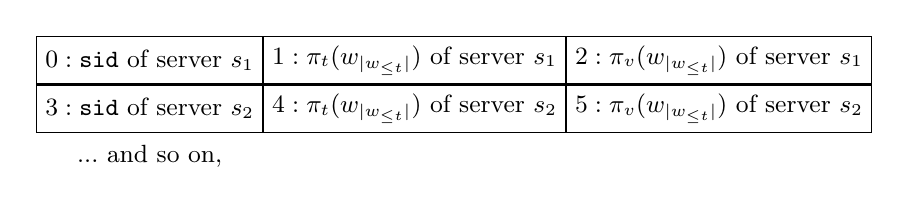
\begin{tikzpicture}
\small
\matrix[nodes={minimum size=6mm}] {
  \node[draw] {$0:\texttt{sid}\textrm{ of server }s_1$};
 &\node[draw] {$1:\pi_t(w_{|w_{\leq t}|})\textrm{ of server }s_1$};
 &\node[draw] {$2:\pi_v(w_{|w_{\leq t}|})\textrm{ of server }s_1$};\\
  \node[draw] {$3:\texttt{sid}\textrm{ of server }s_2$};
 &\node[draw] {$4:\pi_t(w_{|w_{\leq t}|})\textrm{ of server }s_2$};
 &\node[draw] {$5:\pi_v(w_{|w_{\leq t}|})\textrm{ of server }s_2$};\\
  \node {$...$ and so on,};\\
};
\end{tikzpicture}

\noindent
where $\pi_t(w_{|w_{\leq t}|})$ gives the time component of a server's
last-visited waypoint, and $\pi_v(w_{|w_{\leq t}|})$ gives the vertex
component.

\nwenddocs{}\nwbegincode{33}\sublabel{NW3zOIuJ-1bwZd1-1}\nwmargintag{{\nwtagstyle{}\subpageref{NW3zOIuJ-1bwZd1-1}}}\moddef{Filter locs by haversine distance~{\nwtagstyle{}\subpageref{NW3zOIuJ-1bwZd1-1}}}\endmoddef\nwused{\\{NW3zOIuJ-1eKCCy-1}}
public int[] filterByHaversine(int ro, int[] locs, int threshold) \{
  int n = (locs.length/3);
  int[] temp = new int[n];
  int i = 0;
  for (int k = 0; k < n; k++) \{
    if (computeHaversine(ro, locs[((3*k) + 2)]) < threshold) \{
      temp[i++] = 3*k;
    \}
  \}
  return Arrays.copyOf(temp, i);
\}
\nwindexdefn{filterByHaversine}{filterByHaversine}{NW3zOIuJ-1bwZd1-1}\eatline
\nwidentdefs{\\{{filterByHaversine}{filterByHaversine}}}\nwidentuses{\\{{computeHaversine}{computeHaversine}}}\nwindexuse{computeHaversine}{computeHaversine}{NW3zOIuJ-1bwZd1-1}\nwendcode{}\nwbegindocs{34}\nwdocspar
\subsection{{\tt{}\protect\nwindexuse{printUser}{printUser}{NW3zOIuJ-3sWW32-1}printUser}(1)}
The {\tt{}\protect\nwindexuse{printUser}{printUser}{NW3zOIuJ-3sWW32-1}printUser}(1) method can be used to print properties of a ridesharing
user.
\nwenddocs{}\nwbegincode{35}\sublabel{NW3zOIuJ-3sWW32-1}\nwmargintag{{\nwtagstyle{}\subpageref{NW3zOIuJ-3sWW32-1}}}\moddef{Print user~{\nwtagstyle{}\subpageref{NW3zOIuJ-3sWW32-1}}}\endmoddef\nwused{\\{NW3zOIuJ-1eKCCy-1}}
public void printUser(int[] u) \{
  System.out.println("User \{uid="+u[0]+", q="+u[1]+", e="+u[2]+", l="+u[3]
    +", o="+u[4]+", d="+u[5]+", b="+u[6]+"\}");
\}
\nwindexdefn{printUser}{printUser}{NW3zOIuJ-3sWW32-1}\eatline
\nwidentdefs{\\{{printUser}{printUser}}}\nwendcode{}\nwbegindocs{36}\nwdocspar
\subsection{{\tt{}\protect\nwindexuse{printPath}{printPath}{NW3zOIuJ-3QvbXQ-1}printPath}(1)}
The {\tt{}\protect\nwindexuse{printPath}{printPath}{NW3zOIuJ-3QvbXQ-1}printPath}(1) method can be used to print a path.
\nwenddocs{}\nwbegincode{37}\sublabel{NW3zOIuJ-3QvbXQ-1}\nwmargintag{{\nwtagstyle{}\subpageref{NW3zOIuJ-3QvbXQ-1}}}\moddef{Print path~{\nwtagstyle{}\subpageref{NW3zOIuJ-3QvbXQ-1}}}\endmoddef\nwused{\\{NW3zOIuJ-1eKCCy-1}}
public void printPath(int[] p) \{
  for (Integer i : p) \{
    System.out.print(i+" ");
  \}
  System.out.println();
\}
\nwindexdefn{printPath}{printPath}{NW3zOIuJ-3QvbXQ-1}\eatline
\nwidentdefs{\\{{printPath}{printPath}}}\nwendcode{}\nwbegindocs{38}\nwdocspar
\subsection{{\tt{}\protect\nwindexuse{printRoute}{printRoute}{NW3zOIuJ-2sTsm3-1}printRoute}(1)}
The {\tt{}\protect\nwindexuse{printRoute}{printRoute}{NW3zOIuJ-2sTsm3-1}printRoute}(1) method can be used to print a route.
\nwenddocs{}\nwbegincode{39}\sublabel{NW3zOIuJ-2sTsm3-1}\nwmargintag{{\nwtagstyle{}\subpageref{NW3zOIuJ-2sTsm3-1}}}\moddef{Print route~{\nwtagstyle{}\subpageref{NW3zOIuJ-2sTsm3-1}}}\endmoddef\nwused{\\{NW3zOIuJ-1eKCCy-1}}
public void printRoute(int[] w) \{
  for (int i = 0; i < (w.length - 1); i += 2) \{
    System.out.print("("+w[i]+", "+w[(i + 1)]+") ");
  \}
  System.out.println();
\}
\nwindexdefn{printRoute}{printRoute}{NW3zOIuJ-2sTsm3-1}\eatline
\nwidentdefs{\\{{printRoute}{printRoute}}}\nwendcode{}\nwbegindocs{40}\nwdocspar
\subsection{{\tt{}\protect\nwindexuse{printSchedule}{printSchedule}{NW3zOIuJ-45oGvT-1}printSchedule}(1)}
The {\tt{}\protect\nwindexuse{printSchedule}{printSchedule}{NW3zOIuJ-45oGvT-1}printSchedule}(1) method can be used to print a schedule.
\nwenddocs{}\nwbegincode{41}\sublabel{NW3zOIuJ-45oGvT-1}\nwmargintag{{\nwtagstyle{}\subpageref{NW3zOIuJ-45oGvT-1}}}\moddef{Print schedule~{\nwtagstyle{}\subpageref{NW3zOIuJ-45oGvT-1}}}\endmoddef\nwused{\\{NW3zOIuJ-1eKCCy-1}}
public void printSchedule(int[] b) \{
  for (int i = 0; i < (b.length - 3); i += 4) \{
    System.out.print("("+b[i]+", "+b[(i + 1)]
      + ", "+b[(i + 2)]+", "+b[(i + 3)]+") ");
  \}
  System.out.println();
\}
\nwindexdefn{printSchedule}{printSchedule}{NW3zOIuJ-45oGvT-1}\eatline
\nwidentdefs{\\{{printSchedule}{printSchedule}}}\nwendcode{}

\nwixlogsorted{c}{{..round to nearest meter}{NW3zOIuJ-1p0YRJ-1}{\nwixu{NW3zOIuJ-1XfngC-1}\nwixd{NW3zOIuJ-1p0YRJ-1}}}%
\nwixlogsorted{c}{{\code{}Tools\edoc{} definition}{NW3zOIuJ-1xm30x-1}{\nwixu{NW3zOIuJ-2Vh5vZ-1}\nwixd{NW3zOIuJ-1xm30x-1}}}%
\nwixlogsorted{c}{{Compute duration}{NW3zOIuJ-1P2T7X-1}{\nwixu{NW3zOIuJ-1eKCCy-1}\nwixd{NW3zOIuJ-1P2T7X-1}}}%
\nwixlogsorted{c}{{Compute haversine}{NW3zOIuJ-1XfngC-1}{\nwixu{NW3zOIuJ-1eKCCy-1}\nwixd{NW3zOIuJ-1XfngC-1}\nwixd{NW3zOIuJ-1XfngC-2}}}%
\nwixlogsorted{c}{{Compute route}{NW3zOIuJ-20ipbT-1}{\nwixu{NW3zOIuJ-1eKCCy-1}\nwixd{NW3zOIuJ-20ipbT-1}}}%
\nwixlogsorted{c}{{Compute shortest path}{NW3zOIuJ-1XAjSF-1}{\nwixu{NW3zOIuJ-1eKCCy-1}\nwixd{NW3zOIuJ-1XAjSF-1}}}%
\nwixlogsorted{c}{{Compute shortest path distance}{NW3zOIuJ-1A9hi2-1}{\nwixu{NW3zOIuJ-1eKCCy-1}\nwixd{NW3zOIuJ-1A9hi2-1}}}%
\nwixlogsorted{c}{{Filter locs by haversine distance}{NW3zOIuJ-1bwZd1-1}{\nwixu{NW3zOIuJ-1eKCCy-1}\nwixd{NW3zOIuJ-1bwZd1-1}}}%
\nwixlogsorted{c}{{Load GTree}{NW3zOIuJ-b7Jka-1}{\nwixu{NW3zOIuJ-1eKCCy-1}\nwixd{NW3zOIuJ-b7Jka-1}}}%
\nwixlogsorted{c}{{Member variables}{NW3zOIuJ-aPohW-1}{\nwixu{NW3zOIuJ-1xm30x-1}\nwixd{NW3zOIuJ-aPohW-1}}}%
\nwixlogsorted{c}{{Print path}{NW3zOIuJ-3QvbXQ-1}{\nwixu{NW3zOIuJ-1eKCCy-1}\nwixd{NW3zOIuJ-3QvbXQ-1}}}%
\nwixlogsorted{c}{{Print route}{NW3zOIuJ-2sTsm3-1}{\nwixu{NW3zOIuJ-1eKCCy-1}\nwixd{NW3zOIuJ-2sTsm3-1}}}%
\nwixlogsorted{c}{{Print schedule}{NW3zOIuJ-45oGvT-1}{\nwixu{NW3zOIuJ-1eKCCy-1}\nwixd{NW3zOIuJ-45oGvT-1}}}%
\nwixlogsorted{c}{{Print user}{NW3zOIuJ-3sWW32-1}{\nwixu{NW3zOIuJ-1eKCCy-1}\nwixd{NW3zOIuJ-3sWW32-1}}}%
\nwixlogsorted{c}{{Public methods}{NW3zOIuJ-1eKCCy-1}{\nwixu{NW3zOIuJ-1xm30x-1}\nwixd{NW3zOIuJ-1eKCCy-1}}}%
\nwixlogsorted{c}{{Register edges}{NW3zOIuJ-3Nu1Fg-1}{\nwixu{NW3zOIuJ-1eKCCy-1}\nwixd{NW3zOIuJ-3Nu1Fg-1}}}%
\nwixlogsorted{c}{{Register users}{NW3zOIuJ-UKHEr-1}{\nwixu{NW3zOIuJ-1eKCCy-1}\nwixd{NW3zOIuJ-UKHEr-1}}}%
\nwixlogsorted{c}{{Register vertices}{NW3zOIuJ-2ZKKW-1}{\nwixu{NW3zOIuJ-1eKCCy-1}\nwixd{NW3zOIuJ-2ZKKW-1}}}%
\nwixlogsorted{c}{{Tools.java}{NW3zOIuJ-2Vh5vZ-1}{\nwixd{NW3zOIuJ-2Vh5vZ-1}}}%
\nwixlogsorted{c}{{Tools.java preamble}{NW3zOIuJ-1ANZ96-1}{\nwixu{NW3zOIuJ-2Vh5vZ-1}\nwixd{NW3zOIuJ-1ANZ96-1}}}%
\nwixlogsorted{i}{{computeHaversine}{computeHaversine}}%
\nwixlogsorted{i}{{computeRoute}{computeRoute}}%
\nwixlogsorted{i}{{computeShortestPath}{computeShortestPath}}%
\nwixlogsorted{i}{{computeShortestPathDistance}{computeShortestPathDistance}}%
\nwixlogsorted{i}{{CSHIFT}{CSHIFT}}%
\nwixlogsorted{i}{{filterByHaversine}{filterByHaversine}}%
\nwixlogsorted{i}{{flag{\char95}gtree{\char95}loaded}{flag:ungtree:unloaded}}%
\nwixlogsorted{i}{{gtree}{gtree}}%
\nwixlogsorted{i}{{loadGTree}{loadGTree}}%
\nwixlogsorted{i}{{lu{\char95}edges}{lu:unedges}}%
\nwixlogsorted{i}{{lu{\char95}users}{lu:unusers}}%
\nwixlogsorted{i}{{lu{\char95}vertices}{lu:unvertices}}%
\nwixlogsorted{i}{{printPath}{printPath}}%
\nwixlogsorted{i}{{printRoute}{printRoute}}%
\nwixlogsorted{i}{{printSchedule}{printSchedule}}%
\nwixlogsorted{i}{{printUser}{printUser}}%
\nwixlogsorted{i}{{registerEdges}{registerEdges}}%
\nwixlogsorted{i}{{registerUsers}{registerUsers}}%
\nwixlogsorted{i}{{registerVertices}{registerVertices}}%
\nwbegindocs{42}\nwdocspar

\appendix

\section{Appendix: List of Chunks}
\label{ap:list-of-chunks}
\nowebchunks

\section{Appendix: List of Identifiers}
\label{ap:list-of-identifiers}
\nowebindex

\end{document}

\nwenddocs{}
